\chapter{نرم‌افزار}

با این‌که چالش‌های متعددی در مسیر انجام این پروژه خودنمایی کردند، در این فصل صرفا به برخی از چالش‌های مهم‌تر خواهیم پرداخت که می‌توان آن‌ها را در سه دسته‌ی فرآیندی، معماری و محدودیت‌های چارچوبی دسته‌بندی کرد.

\section{؟}

%\subsection{ترکیب فرآیندهای ظاهر و باطن سامانه}

یکی از مهم‌ترین چالش‌های فرآیندی که در روال توسعه اسکرام در این پروژه مشخص شد، لزوم جداسازی \lr{Backlog}های ظاهر\footnote{\lr{Front-end}} و باطن\footnote{\lr{Back-end}} سامانه از یکدیگر بود. با توجه به اینکه در این پروژه از سامانه جیرا برای مدیریت فرآیند توسعه استفاده می‌شود، در ابتدا برای هر استوری کاربر، دو زیرمجموعه فرانت-اند و بک-اند تعریف شده بود که در عمل مشخص شد این نوع تعریف، کارآیی لازم را ندارد و در فرآیندهای چابک، باعث توسعه ناقص چند اسپرینت و درنهایت تکمیل تعدادی از آن‌ها بصورت یکجا بجای تکمیل هرکدام در ترتیب درست می‌شود.\\

البته این مسئله با رعایت دقیق تقدم‌ها و تاخرها تاحدی قابل پیش‌بینی است، اما نکته مهم در این‌جا، چابک بودن روال توسعه است (در مقابل برنامه‌محوری\footnote{\lr{Plan-driven}})؛ پس تقدم و تاخر پیش‌بینی شده لزوما محقق نخواهد شد و اگر در اواسط کار، نیازمندی‌ها تغییرکنند و یا زوایای پنهانی از سامانه شناسایی شود، حتما این مورد می‌تواند مشکل‌ساز باشد. بنابراین اگر روال توسعه سنتی بود و از یک برنامه دقیق و غیرقابل انعطاف استفاده می‌شد شاید هرگز چنین چالشی بوجود نمی‌آمد، اما در آن شرایط کل روال اسکرام زیرسوال می‌رفت و دیگر کاربردی نداشت!\\

\newpage

%\subsection{ترکیب فرآیندهای نقش‌های مختلف کاربران}

یک چالش دیگر، مرکب بودن انواع نقش‌های کاربران در یک اسپرینت\footnote{\lr{Sprint}} بود. برای مثال در استوری‌های تعریف شده برای اسپرینت دوم از فرآیند توسعه، هم برای نقش فروشنده استوری کاربر تعریف شده و هم برای نقش خریدار. با توجه به این‌که برای بسیاری از بخش‌ها، حتما باید یک نقش تا حد مشخصی تکمیل شود و سپس توسعه نقش دیگر آغاز شود، این تقسیم‌بندی نیز می‌تواند باعث توسعه ناقص ولی همزمان چند اسپرینت شود. بنابراین، تنها توجه به تقدم و تاخر پیاده‌سازی‌ها کافی نیست و باید تا جای ممکن از ترکیب نقش‌های مختلف کاربران در یک اسپرینت پرهیز شود (مگر این‌که از لحاظ منطقی مشکلی برای تقدم و تاخرهای پیش‌بینی شده ایجاد نکند).\\

%\subsection{تولید داده‌های آزمون}

یکی دیگر از چالش‌ها، لزوم مشخص کردن آزمون‌های سطح سیستم (و نه صرفا آزمون‌های واحد) در \lr{Backlog}هاست. با توجه به اینکه برای آزمون انسانی و دستی هر بخش از این سامانه به حجم قابل توجهی از داده‌های تست نیاز داریم، تولید این حجم از داده‌های آزمون بصورت دستی امکان‌پذیر نیست؛ بنابراین لازم است تا بخشی تحت عنوان آزمون‌های سطح سیستم از همان ابتدای توسعه شکل بگیرد و پیش‌اجراهایی برای آزمون‌های سیستمی از ابتدا نوشته شود که در آن‌ها، تعداد مناسبی از داده‌های آزمون بطور خودکار تولید شده و برای آزمون‌های انسانی آتی و یا حتی خود آزمون‌های سیستمی خودکار مورد استفاده قرار بگیرند.\\

چالش گفته شده را نباید با روال طبیعی آزمون‌های خودکار اشتباه گرفت. مجددا تاکید می‌شود که داده‌های تولید شده برای آزمون را نمی‌توان بصورت دستی و انسانی در این حجم ایجاد کرد و حتما بایستی بصورت خودکار ساخته شوند؛ اما استفاده از این داده‌ها لزوما خودکار نخواهد بود. بنابراین نه تنها آزمون خودکار، بلکه آزمون اولیه دستی نیز به این داده‌ها برای تحقق خود نیاز خواهد داشت.\\

\newpage

%\subsection{تمرکز بیشتر بر طراحی دنباله درخواست‌ها}

اگر این پروژه بخواهد در یک محیط صنعتی و با شرایط زمانی گسترده‌تر از حالت فعلی انجام بپذیرد، حتما باید مدت زمان و \lr{Backlog}های بیشتری به بحث طراحی، بخصوص طراحی روند ارتباط فرانت-اند و بک-اند و دنباله درخواست‌ها و پاسخ‌های ارسالی و دریافتی برای انجام عملیات‌های اصلی سامانه اختصاص یابد. (منظور از روند ارتباط، معرفی نقاط دسترسی نهایی (یا همان اندپوینت\footnote{\lr{Endpoint}}‌ها) و جزئیات آن‌ها نیست. بلکه هر عملکرد معنایی در این سامانه، شامل دنباله‌ای از درخواست‌های شبکه می‌شود که به ترتیب پشت سر هم اجرا شده و ممکن است هر یک برای اجرای خود از داده‌های خروجی قبلی استفاده نماید.)\\

برای مثال، در اواخر فصل قبلی درمورد روال دو مرحله‌ای ورود و ثبت‌نام کاربران در سامانه توضیح داده شد. این روال درواقع یکی از همین دنباله‌هاست که مشخص بودن آن حتی پیش از طراحی مدل‌داده‌ها (و یا همزمان با آن) می‌تواند باعث تغییرات بنیادی در طراحی آن شود. همچنین اگر این طراحی‌ها مشخص باشد می‌توان به بخشی از چالش اول گفته شده (ترکیب فرآیندهای ظاهر و باطن سامانه) نیز غلبه کرد؛ زیرا درآن‌صورت، فعالیت‌هایی که یکی از ظواهر سامانه (مثلا نرم‌افزار کاربردی تلفن هوشمند) برای انجام یک عملیات خاص باید انجام دهد و دنباله درخواست‌هایی که باید به باطن سامانه (که همان سامانه اصلی است) مشخص خواهد بود و تقدم و تاخر در طراحی هرکدام نسبت به یکدیگر مستقل خواهد بود.

%\section{چالش‌های معماری}

%\subsection{انتقال تغییرات داده به لایه‌های بیرونی در ری‌اکت}

یکی از مهم‌ترین چالش‌هایی که با معماری انتقال داده‌ها درون نرم‌افزار کاربردی این سامانه (که با ری‌اکت پیاده‌سازی شده است) وجود داشت،‌ مسئله بازتاب تغییرات داده‌ها در لایه‌های بیرونی نرم‌افزار (و صفحات قبلی و عمومی‌تر) و درادامه، انتقال تغییرات به سامانه اصلی بود. به این‌صورت که اگر از صفحه لیست فروشگاه‌ها وارد صفحه یک فروشگاه شده، و از لیست محصولات آن وارد صفحه تغییر اطلاعات یک محصول شویم و اطلاعات آن را تغییر بدهیم، اطلاعات وارد شده باید درهنگام برگشت از صفحه تغییرات، در لیست محصولات اعمال شده باشد.

با معماری که در ابتدا استفاده شده بود تغییرات بلافاصله در لیست محصولات اعمال نمی‌شد و حتما باید یکبار لیست محصولات بسته و دوباره باز می‌شد. در واقع‌ معماری استفاده شده برای ذخیره داده‌های فروشگاهی در ابتدا، برای تغییر داده‌های مذکور، لیست جدید تمام داده‌های زیرمجموعه فروشگاه‌های یک فروشنده را در ورودی دریافت می‌کرد و کل آن‌ها را بازنویسی می‌کرد. شاید فقط یک خصوصیت مختصر از یکی از محصولات تغییر کرده بود، اما برای تغییر همان یک خصوصیت باید تمامی فروشگاه‌های کاربر بروزرسانی می‌شدند.

چون درون صفحات داخلی، به اطلاعات صفحات بیرونی دسترسی کاملی وجود ندارد،‌ عملا ایجاد این دسترسی سربار زیادی برای ساختار طبیعی یک نرم‌افزار تحت چارچوب ری‌اکت نیتیو ایجاد می‌کرد. علاوه بر این، خصوصیاتی از مدل داده‌های مربوط به فروشگاه‌های یک فروشنده بودند که عملا توسط نرم‌افزار کاربردی دریافت نمی‌شدند و صرفا توسط سامانه اصلی مدیریت شده ولی در پایگاه‌داده موجود بودند؛ پس عملا بازنویسی کل این لیست توسط نرم‌افزار کاربردی سامانه، باعث پاک شدن تمام آن اطلاعات می‌شد!

بنابراین، این شیوه حتما باید تغییر می‌کرد. برای حل این چالش، برای هرکدام از موجودیت‌های مرتبط با یک فروشنده (از جمله فروشگاه، محصول و کوپن تخفیف) یک گره\footnote{\lr{Node}} جداگانه در گرف‌کیوال تعریف شد که فقط خصوصیات اولیه\footnote{\lr{Primitive}} آن موجودیت را تغییر می‌داد و تنظیم می‌کرد. برای خصوصیاتی که لیست و آرایه بودند، مانند محصولات یک فروشگاه، سه گره جداگانه ایجاد شد که هرکدام یکی از سه وظیفه ایجاد\footnote{\lr{Create}}، ویرایش\footnote{\lr{Edit}} و حذف\footnote{\lr{Delete}} یک عضو از آن آرایه را انجام می‌دادند.

\begin{figure}[H]
	\centering
	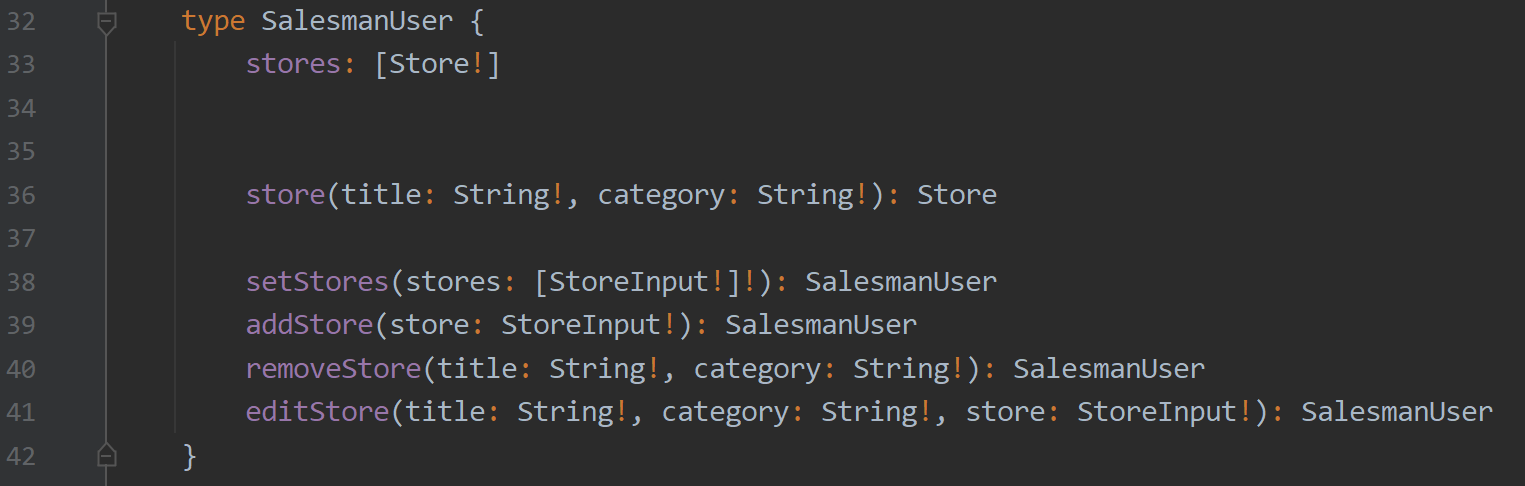
\includegraphics[scale=0.55]{rnch}
	\caption{گره‌های تعریف شده در گرف‌کیوال برای ویرایش آرایه محصولات از یک فروشنده}
	\label{fig:rnch}
\end{figure}

برای گره‌های ویرایش و حذف، حتما باید مشخص می‌شد که منظور ما کدام عضو از آن موجودیت است. مثلا برای حذف یک محصول از درون لیستی از محصولات یک فروشگاه، باید مشخص باشد آن محصول کدام عضو آن لیست است. چه برای فروشگاه‌ها و چه برای محصولات، فرض شده که هیچ دو محصولی در یک فروشگاه، و هیچ دو فروشگاهی برای یک فروشنده وجود ندارند که نام و دسته‌بندی آن‌ها یکسان باشد. بنابراین از لحاظ مفهومی، زوج خصوصیت \{نام، دسته‌بندی\} بعنوان یک کلید اولیه\footnote{\lr{Primary‌ Key}} از هر محصول یا فروشگاه انتخاب شدند. در \cref{fig:rnch} نیز برای گره \lr{removeStore} مطلب اخیر قابل مشاهده است.

از طرفی دیگر درون نرم‌افزار پیاده‌شده با ری‌اکت نیتیو، روش مرسوم ایجاد تغییرات در داده‌ها از صفحات داخلی‌تر به صفحات بیرونی‌تر است. اما باتوجه به مشکلات ذکر شده در این پروژه از این روش استفاده نشده؛ بلکه تغییرات درهیچ یک از صفحات بصورت محلی در ابتدا اعمال نمی‌شوند و از طریق بیرونی‌ترین صفحه به سامانه اصلی (از طریق درخواست گرف‌گیوال) ارسال می‌شوند. اگر سامانه اصلی آن را تایید کند، این استاندارد رعایت شده که سامانه اصلی همواره شی یک سطح بالاتر از نقطه تغییرات را (پس از اعمال تغییرات جدید) بازگرداند. بنابرین صفحه بیرونی این شی جدید را دریافت کرده و سپس اقدام به تغییر کل وضعیت\footnote{\lr{State (useState Hook)}} داخلی از خودش می‌کند و این تغییر با استفاده از یک محتوا\footnote{\lr{Context (useContext Hook)}} در ریکعت نیتیو، به اطلاع تمامی صفحات داخلی‌تر می‌رسد و آن‌ها نیز داده جدید را دریافت می‌کنند\cite{react:hooks}.

%\subsection{تنظیم سطح شفافیت و دسترسی در گرف‌کیوال}

در مدل نوشته برای گرف‌کیوال، تمام داده‌ها از لحاظ شفافیت و سطوح دسترسی، یکسان و در یک سطح دیده می‌شوند. اما برای مثال، شماره تلفن همراه برخی از کاربران نباید برای کاربران دیگر قابل دریافت باشد! از طرفی،‌ اگر این محدودیت دسترسی را بخواهیم در نرم‌افزار کاربردی سامانه پیاده‌سازی کنیم ساده‌انگارانه خواهد بود و از لحاظ امنیت اطلاعات راهکار پذیرفته شده‌ای نیست؛ درواقع می‌توان گفت این موضوع لازم است اما نه کافی.

همواره باید درنظر داشت که سامانه اصلی می‌تواند توسط هر کاربری فراخوانی شود و لزوما کاربر آن نرم‌افزار کاربردی تلفن هوشمند و یا پنل تحت وب مدیران نخواهد بود. پس این محدودیت‌ها باید صریحا از سمت سامانه اصلی مدیریت و اعمال شوند.

در توابع پیاده‌سازی‌کننده گره‌های گرف‌کیوال، شی‌ای تحت عنوان \lr{Context} در ورودی داده می‌شود که می‌تواند شامل اطلاعات احرازهویت و حساب کاربر اجراکننده درخواست فعلی باشد. از روی این شی می‌توان هویت و سطح دسترسی هر کاربر را درحین درخواست هر یک از گره‌های گرف‌کیوال تعیین کرد و مطابق با آن واکنش نشان داد.

پس در مثالی که مطرح شد، باید برای گره خصوصیت شماره موبایل هر فرد، ابتدا نوع حساب کاربری آن فرد بررسی شود و اگر شرایط موردنیاز فراهم بود،‌شماره برگردانده شود و درغیراین‌صورت،‌ خطای عدم دسترسی\footnote{\lr{Access Denied}} اعلام شود. این عملیات باید در تابع رافع\footnote{\lr{Resolver}} این خصوصیت تعریف شود و بنابراین، گرف‌کیوال دیگر از تابع رافع بدیهی\footnote{\lr{Trivial}} برای این خصوصیت (شماره موبایل) استفاده نخواهد کرد.

در توضیح محتویات شی \lr{Context} باید به شیوه احرازهویت استفاده شده اشاره شود. برای انجام احرازهویت در این سامانه از بلیت‌های \lr{JWT} استفاده شده است. این بلیت‌ها در خود سامانه اصلی و درهنگام تکمیل شدن احرازهویت دومرحله‌ای (که در فصل پیش به آن پرداختیم) ساخته شده و توسط یک زوج کلید نامتقارن 256 بیتی رمزنگاری می‌شود؛ البته این رمزنگاری برای حفظ اصالت بلیت تولیدشده است و نه حفظ محرمانگی. این بلیت در هر درخواست کاربر که احرازهویت نیاز داشته باشد باید تحت سرآیند اچ‌تی‌تی‌پی با مقدار کلید \lr{Authorization} و با مقدار \lr{Bearer TOKEN} که در آن \lr{TOKEN} برابر با بلیت دریافتی قبلی می‌باشد ارسال شود\cite{jwt}. 

%\subsection{پایگاه‌داده اصلی و آزمایشی}

با توجه به این‌که در این سامانه از آزمون‌های خودکار (بخصوص برای تولید داده‌های نمونه) استفاده شده، بنابراین باید پایگاه‌داده اصلی آن از پایگاه‌داده آن وقتی درحال اجرای آزمون‌های خودکار است جدا باشد. برای این‌کار راحت‌ترین راه استفاده از دو نام جداگانه برای پایگاه‌داده‌ها در دستور برقراری ارتباط است.\\

اما مشکل از جایی شروع می‌شود که سامانه اصلی برای اجرای خود باید در همان لحظه ابتدای اجرا به پایگاه‌داده متصل شود (زیرا مدل داده‌ها برای اجرا شدن نیاز به ارتباط اولیه با پایگاه‌داده دارد)، از طرفی آزمون‌های خودکار نیز بلافاصله بعد از اجرا شدن کل سامانه، اجرا می‌شوند.

این همزمانی باعث می‌شود بخش اصلی کد، متوجه این نباشد که این اجرای واقعی است و یا جهت آزمایش سامانه! بنابراین باید این بخش آزمون‌ها با سازوکاری به بخش اصلی بفهماند که این اجرا صرفا برای آزمایش است و بخش اصلی باید به پایگاه‌داده آزمایشی متصل شود. خود بخش آزمون نیز باید اجرای آزمون‌ها را به زمان برقراری کامل ارتباط پایگاه‌داده موکول کند.\\

برای حل این چالش، از ترکیب چند ساختار غیرهمزمان‌\footnote{\lr{Asynchronous}}سازی در جاواسکریپت به نام \lr{Promise}ها با یک متغیر محیطی\footnote{\lr{Environment Variable}} استفاده شده است.

%\section{چالش‌های محدودیت چارچوب‌ها}

در این بخش به چالش‌هایی پرداخته شده‌است که ناشی از محدودیت موجود در چارچوب‌های مورد استفاده است. البته چالش‌های بیشتری نیز وجود داشته، ‌اما در این‌جا فقط به ذکر دو مورد مهم از آن‌ها اکتفا می‌شود.

\newpage

%\subsection{مسئله‌ی \lr{N+1} گرف‌کیوال}

این مشکل وقتی اتفاق می‌افتد که در کوئری ارسالی به گرف‌کیوال، چند سطح از  داده درخواست شده باشد که\cite{gql:nplusone}:
\begin{enumerate}
	\item این سطوح هر کدام نیازمند ارتباط با پایگاه‌داده باشند، و
	\item سطح بیرونی، یک آرایه را برگرداند.
\end{enumerate}

در این‌صورت، 1 ارتباط با پایگاه‌داده برای سطح بیرونی و \lr{N} ارتباط نیز به تعداد اعضای آرایه بیرونی برای پر کردن داده سطح دوم تمام اعضای آرایه (که \lr{N} عضو دارد) موردنیاز خواهد بود. درحالی‌که اگر همین مدل را با \lr{REST} پیاده می‌کردیم، فقط به 2 کوئری نیاز داشتیم. یعنی بجای کل \lr{N} کوئری در سطح داخلی، یک کوئری دیگر نیاز بود\cite{gql:nplusone}.

این مسئله، به نوعی جزو مسائل باز حساب می‌شود. دلیل این مسئله، اشتباه بودن گره‌های ایجاد شده برای گرف‌کیوال، و یا استفاده از پایگاه‌های داده \lr{SQL} است! درواقع وقتی از این نوع پایگاه‌های داده برای گرف‌کیوال استفاده شود، احتمال رخداد چنین چالشی بسیار بیشتر از زمانی است که از پایگاه‌داده مونگو استفاده می‌شود.\\

راه‌حل این مشکل زمانی‌که از اس‌کیوال‌ها استفاده شود، تجمیع کوئری‌های پایگاه‌داده از درون سطوح داخلی گره‌های گرف‌کیوال بهمراه سطوح خارجی، و اجرای یکباره‌ی آن‌هاست. برای این‌کار می‌توان از کتابخانه دیتالودر\footnote{\lr{ِDataloader}} که توسط خود سازنده گرف‌کیوال طراحی و پیاده‌سازی شده است استفاده کرد.

اما در این پروژه، باتوجه به این‌که از پایگاه‌داده مونگو استفاده شده، سعی شده که در تمام نقاط و گره‌های گرف‌کیوال، داده‌های موردنیاز در همان سطح بیرونی از مونگو گرفته شود و در سطوح داخلی، صرفا خصوصیات آن اشیا انتخاب شده و برگردانده شوند و به لطف مدل داده‌ی تودرتوی این پروژه، نیاز به پرس‌وجوی مجدد از پایگاه‌داده در سطوح داخلی گرف‌کیوال وجود نداشته باشد.

درواقع و از دیدگاه پیاده‌سازی، دو گره اصلی \lr{me} و \lr{baseUser} نقطه اصلی اتصال گرف‌کیوال به پایگاه‌داده است و در این دو گره، شی کاربر موردنظر بطور کامل از پایگاه‌داده دریافت می‌شود و بجز برای اعمال تغیرات، دسترسی دیگری به پایگاه‌داده در سطوح داخلی‌تر ایجاد نخواهد شد و پس از آن، صرفا از خصوصیات متغیرهای موجود درحافظه استفاده می‌شود. 

\newpage

%\subsection{مرتب‌سازی طبق فاصله مکانی در مونگو}

از مهم‌ترین ویژگی‌های این سامانه، کار آن با موقعیت‌های مکانی و مختصات‌های جغرافیایی است. یکی از دلایل انتخاب پایگاه‌داده مونگو برای این پروژه نیز همین بوده است؛ زیرا مونگو امکانات وسیعی را در حوزه کار با مختصات جغرافیایی بطور پیشفرض فراهم می‌کند. برای مثال، تمامی اشیا مختصات درون یک مجموعه\footnote{\lr{Collection}} را فهرست\footnote{\lr{Index}} می‌کند تا در پرس‌وجوها، بسیار سریع به آن‌ها دست پیدا کند.

قابلیت اخیر ذکر شده، امکان جستجوی اسناد\footnote{\lr{Documents}}ی که درآن‌ها مختصات نزدیک‌تری به یک نقطه خاص وجود دارد در مدت زمان بسیار کوتاهی فراهم می‌کند. حتی اگر مجموعه اسناد بسیار زیاد و در مقیاس چند ده هزار عدد باشند، باز هم جستجو به لطف عملیات فهرست که روی مختصات در هنگام اضافه شدن آن‌ها به مجموعه انجام شده است، در مدت زمانی با مقیاس میلی‌ثانیه انجام خواهد شد.\\

در این‌جا لازم است مفاهیم استفاده شده را برای فهم بهتر مسئله به معادل اس‌کیوال آن نظیر کنیم. مجموعه در مونگو،‌ همان جدول و سند، همان ردیف جداول در اس‌کیوال هستند. اشیا و کلیدهای داخلی یک سند در مونگو، همان ستون‌ها و درمقیاس یک ردیف، معادل همان سلول‌های یک جدول در اس‌کیوال می‌باشند.

همان‌طور که در فصل دوم و در توضیح مفاهیم پایه مونگو گفته شد، این پایگاه‌داده از نوعی دستورات به نام دستورات تجمیع\footnote{\lr{Aggregation}} استفاده می‌کند. این دستورات در واقع مجموعه‌ای از مراحل تجمیع را درون خود دارند که در حین اجرای آن، مونگو کل داده‌های درون مجموعه را بعنوان ورودی اولین مرحله وارد آن می‌کند و خروجی مرحله اول تولید می‌شود؛ سپس خروجی تولید شده بعنوان ورودی وارد مرحله دوم می‌شود و همین روال تا مرحله آخر ادامه پیدا می‌کند. خروجی تولید شده از مرحله آخر،‌ بعنوان خروجی کل دستور تجمیع شناخته شده و بازگردانده می‌شود. درواقع این مراحل یک نوع خط لوله\footnote{\lr{Pipeline}} هستند و با نام مراحل خط لوله تجمیع در مونگو شناخته می‌شوند.

\newpage

دستورات مختلفی بعنوان مراحل خط لوله تجمیع در مونگو وجود دارند. اما دستور مهمی که چالش پیشِ‌رو را ایجاد کرده است،‌ دستور خط لوله \lr{\$GeoNear} است. این دستور بر روی یک کلید دارای شی مختصات از هر سند اعمال می‌شود و اسناد خروجی را به ترتیب فاصله (از نزدیک به دور) از یک نقطه ثابت داده شده مرتب می‌کند. این دستور خط لوله یک محدودیت بسیار مهم دارد و آن، اجبار مونگو در اولین مرحله بودن این دستور از خط لوله تجمیع است. پس برای استفاده از این دستور حتما باید آن را در اولین مرحله از خط لوله تجمیع اجرایی قرار داد\cite{mongo:geo}. این موضوع به خودیِ‌خود مشکلی ایجاد نمی‌کند و تنها یک محدودیت معقول مراحل خط لوله تجمیع در مونگو است.\\

مشکل اول وقتی ایجاد می‌شود که درون یک سند از مجموعه، آرایه‌ی مستقیم یا غیرمستقیمی از اشیا مختصات داشته باشیم. در مدل داده‌های این سامانه، هر کاربر یک سند داده خواهد داشت. بنابراین اگر آن کاربر فروشنده باشد، آرایه‌ای از فروشگاه‌ها خواهد داشت و هر فروشگاه نیز یک مختصات و موقعیت مکانی مخصوص به خود دارد. پس در این‌جا نیز هر سند فروشنده از مجموعه اصلی سامانه، شامل آرایه‌ای از مختصات‌ها خواهد بود. مشکل این است که خروجی دستور خط لوله \lr{\$GeoNear} به ازای هر سند، یک سند خواهد بود؛ حتی اگر آن سند دارای آرایه‌ای از مختصات باشد. پس معلوم نمی‌شود که برای یک فروشنده، کدام فروشگاه به خریدار نزدیک‌تر بوده و فقط کل فروشگاه‌های آن فروشنده بازگردانده می‌شود.\\

البته دستور \lr{\$GeoNear} در نسخه‌های آخر مونگو، کلیدی را درخروجی اضافه کرده که صریحا مشخص می‌کند درصورت آرایه بودن مختصات‌ها، کدام یکی از آن‌ها نزدیک‌ترین به نقطه ثابت داده شده بوده است، اما ترتیب مختصات دیگر را (بجز نزدیک‌ترین مختصات درون آرایه‌های مختصات همان یک سند) اصلاح نمی‌کند\cite{mongo:geo}؛ بنابراین مشکل قبلی که گفته شد در نسخه‌های آخر مونگو رفع شده است، اما همچنان این مشکل جدید وجود خواهد داشت. درواقع اگر یک فروشنده 3 فروشگاه داشته باشد، فقط نزدیک‌ترین آن‌ها به مشتری مشخص می‌شود و بین 2 فروشگاه دیگر ترتیب مکانی نامشخص خواهد بود.

چالش اخیر ذکر شده را براحتی می‌توان درون سامانه اصلی (بیرون از دستورات بومی پایگاه‌داده) و یا حتی در نرم‌افزار کاربردی در سمت کاربر رفع کرد. زیرا هر فروشنده تعداد زیادی فروشگاه نخواهد داشت و زمان محاسبه موردنیاز برای مرتب کردن فروشگاه‌های یک فروشنده زیاد نخواهد بود و در مقیاس میلی‌ثانیه انجام خواهد شد.

\newpage

اما این تنها مشکل و چالش نیست؛ ما مطمئن نیستیم که اگر فروشگاه‌های هر فروشنده را جداگانه مرتب کنیم، و آن‌گاه خود فروشنده‌ها را طبق فروشگاه‌های اول هر فروشنده (که نزدیک‌ترین از هرکدام خواهد بود) مرتب نماییم، خروجی ایجاد شده کاملا صحیح باشد! زیرا ممکن است فروشگاه دوم  فروشنده دوم، از فروشگاه دوم فروشنده اول،‌ به نقطه ثابت داده شده (که موقعیت خریدار است) نزدیک‌تر باشد! هرچند این اتفاق به ندرت ممکن است رخ دهد و بخصوص وقتی خروجی درون یک لیست بزرگ نمایش داده شود، شاید اشتباه بودن یک ترتیب در عناصر داخلی آن لیست برای کاربری که درحال مشاهده تمام آن‌ها در همان لحظه و بصورت یکجا است چندان اهمیتی نداشته باشد، اما بهرحال اگر بصورت تئوری به مسئله نگاه شود، این موضوع یک نقص و چالش است.

برای حل این چالش، بهترین راهی که بنظر می‌رسد، باز و پخش کردن فروشگاه‌ها از آرایه‌های فروشنده‌ها و همسطح کردن تمام آن‌ها از طریق دستور مرحله خط لوله تجمیع \lr{\$Unwind} است. اما آن محدودیت اولیه که از دستور \lr{\$GeoNear} گفته شد، این‌جا مشکل‌ساز می‌شود! طبق این محدودیت مونگو،‌ نمی‌توان از یک مرحله \lr{\$Unwind} پیش از مرحله \lr{\$GeoNear} استفاده کرد. پس عملا این راه‌حل ناممکن خواهد بود!\cite{mongo:geostack}\\

برای این چالش راه‌حل‌هایی وجود دارند که بسیار پرهزینه هستند؛ مثل اصلاح نقوص احتمالی حاصل از جستجو و مرتب‌سازی بدون درنظرگرفتن این مشکل، در سامانه اصلی و یا در نرم‌افزار کاربردی. چون تعداد کل فروشگاه‌ها بسیار بالاست این عملیات قطعا از پیچیدگی زمانی بالایی برخوردار خواهد بود و گلوگاه\footnote{\lr{Bottleneck}} محاسبات مرتب‌سازی این سامانه خواهد شد. بنابراین تکیه بر نرم‌افزار کاربردی سامانه برای حل این چالش منطقی نخواهد بود.

بهترین راهی که برای حل این مسئله در تحقیقات و بررسی‌های انجام شده یافت شد، ایجاد یک مجموعه (معادل جدول) موقت از خروجی‌های مرتب‌سازی عادی در این مرحله (بدون توجه به این چالش و با استفاده از \lr{\$Unwind} بعنوان اولین مرحله خط لوله)، و سپس استفاده از یک \lr{\$GeoNear} بر روی مجموعه موقت ایجاد شده (در قالب یک خط لوله جدید) و درنهایت حذف مجموعه موقت است. البته بجز این روش، می‌توان مدل‌داده‌ها را تغییر داد و فروشگاه‌ها را بصورت یک مجموعه جداگانه ارائه کرد (که البته هزینه این روش در اثر تاثیرات این تغییر روی مابقی الگوریتم‌ها ممکن است بیشتر از هزینه روش قبلی باشد!).

با پیاده‌سازی راه‌حلی که گفته شد (استفاده از مجموعه موقت و دومرحله‌ای کردن مرتب‌سازی)، زمان پاسخ‌دهی سامانه برای تعداد بالایی خروجی از فروشگاه‌ها تقریبا 3 برابر شد (از حدود 150 میلی‌ثانیه به 400 میلی‌ثانیه) که البته با توجه به این‌که در عمل تمامی فروشگاه‌ها خروجی داده نمی‌شوند و تعداد آن‌ها با استفاده از مکانیزم‌های صفحه‌بندی\footnote{\lr{Pagination}} خروجی کمتر از این حالت خواهد بود، تاخیر قابل قبولی است و در عوض، خروجی مرتب‌سازی طبق موقعیت مکانی، بدون هیچ‌گونه نقص منطقی ارائه می‌شود.

